\documentclass[a4paper]{article}

\usepackage{fullpage} % Package to use full page
\usepackage{parskip} % Package to tweak paragraph skipping
\usepackage{amsmath}
\usepackage{amssymb}
\usepackage{hyperref}
\usepackage{subcaption}
\usepackage{graphicx}
\usepackage{fancyvrb}

\title{16-720B Computer Vision: Homework 5 \\
Neural Networks for Recognition}
\author{Heethesh Vhavle\\
Andrew ID: hvhavlen}
\date{22 November 2018\\(Using \textbf{THREE LATE DAYS})}

\begin{document}

\maketitle

\section{Theory}
\subsection{Softmax Translation Invariance}
The proof is as follows. The term $e^{c}$ can be factored out in both the numerator and the denominator.
\begin{equation}
\begin{gathered}
    \operatorname { softmax } \left( x _ { i } \right) = \frac { e ^ { x _ { i } } } { \sum _ { j } e ^ { x _ { j } } } \\
    \operatorname { softmax } \left( x _ { i } + c \right) = \frac { e ^ { x _ { i } + c} } { \sum _ { j } e ^ { x _ { j } + c } } \\
    \operatorname { softmax } \left( x _ { i } + c \right) = \frac { e^{x_{ i }} e^{c} } { e^{c} \sum _ { j } e ^ { x _ { j } } } \\
    \operatorname { softmax } \left( x _ { i } + c \right) = \frac { e ^ { x _ { i } } } { \sum _ { j } e ^ { x _ { j } } } \\
    \therefore \operatorname { softmax } \left( x _ { i } \right) = \operatorname { softmax } \left( x _ { i } + c \right)
\end{gathered}
\end{equation}

By setting $c = - \max x _ { i }$ or subtracting the maximum value exponent term, we get $e^{0}=1$ and all the other terms will be scaled between 0 and 1, thus avoiding large exponent terms which improves numerical stability and avoids overflows.

\subsection{Softmax Properties}
\subsubsection{}
Every element, for $d>2$, will be in the interval (0, 1) and the sum over all elements will be equal to 1.

\subsubsection{}
One could say that \textit{``Softmax takes an arbitrary real valued vector x and turns it into a vector of size (d, 1) with each element of the vector in the interval (0, 1) and sum over all elements equal to 1."}

\subsubsection{}
The first step is the exponential which increases the probability of the biggest score and decreases the probability of the lowest score exponentially, which is much closer to the argmax compared just taking the mean. The second step is to sum up all the probabilities and the final step is to divide all the probabilities by the sum to ensure that the output is in the interval (0, 1) and the sum of all probabilities is 1.

\subsection{Multi-Layer Neural Networks}
Let us consider this network without any activation functions. Let $H_{i}$ be the output at every layer and let $n$ be total number of layers. 

\begin{equation}
\begin{gathered}
    H_{i} = W_{i}H_{i-1} + b_{i} \\
    H_{n} = W_{n}H_{n-1} + b_{n} \\
    H_{n-1} = W_{n-1}H_{n-2} + b_{n-1} \\
    H_{n} = W_{n}(W_{n-1}H_{n-2} + b_{n-1}) + b_{n} \\
    H_{n} = W_{n}W_{n-1}H_{n-2} + (W_{n}b_{n-1} + b_{n})
\end{gathered}
\end{equation}

Similarly, we can express this network for all layers till the input layer as a linear combination of product of the weights added with some bias term, which is essentially the same as linear regression.
\begin{gather}
    H_{n} = W_{n}W_{n-1}W_{n-2} \dots W_{1}X + bias
\end{gather}

Thus, we can see that multi-layer neural networks without a non-linear
activation function are equivalent to linear regression.

\subsection{Sigmoid Derivative}
Differentiating using chain rule, we get the following.
\begin{equation}
\begin{gathered}
    \sigma ( x ) = \frac { 1 } { 1 + e ^ { - x } } = \left( 1 + e ^ { - x } \right) ^ { - 1 } \\
    \frac { d } { d x } \sigma ( x ) = \frac { d } { d x } \left( \left( 1 + e ^ { - x } \right) ^ { - 1 } \right) \\
    \frac { d } { d x } \sigma ( x ) = - 1 \left( \left( 1 + e ^ { - x } \right) ^ { ( - 2 ) } \right) \left( e ^ { - x } \right) ( - 1 ) \\
    \frac { d } { d x } \sigma ( x ) = \frac { \left( e ^ { - x } \right) } { \left( 1 + e ^ { - x } \right) ^ { 2 } }
\end{gathered}
\end{equation}

We can simplify the above, by adding and subtracting 1 in the numerator and rewrite it in terms of $\sigma(x)$.
\begin{equation}
\begin{gathered}
    \frac { d } { d x } \sigma ( x ) = \frac { \left( 1 + e ^ { - x } - 1 \right) } { \left( 1 + e ^ { - x } \right) ^ { 2 } } \\ 
    \frac { d } { d x } \sigma ( x ) = \frac { \left( 1 + e ^ { - x } \right) } { \left( 1 + e ^ { - x } \right) ^ { 2 } } - \frac { 1 } { \left( 1 + e ^ { - x } \right) ^ { 2 } } \\
    \frac { d } { d x } \sigma ( x ) = \frac { 1 } { \left( 1 + e ^ { - x } \right) } \left( 1 - \frac { 1 } { \left( 1 + e ^ { - x } \right) } \right) \\
    \therefore \frac { d } { d x } \sigma ( x ) = \sigma(x) (1-\sigma(x))
\end{gathered}
\end{equation}

\subsection{Gradient of Loss Function}
We have the following.
\begin{equation}
\begin{gathered}
    y = x ^ { T } W + b \\
    y_{j} = x _ { 1 } W _ { 1 j } + b _ { j }  + x _ { 2 } W _ { 2 j } + b _ { j } + \dots + x _ { m } W _ { m j } + b _ { j }\\
\end{gathered}
\end{equation}

We can represent the derivatives with respect to $W$ as follows.
\begin{equation}
\begin{gathered}
    \frac { \partial J } { \partial W } = \frac { \partial J } { \partial y } \frac { \partial y } { \partial W } \\
    where, \frac { \partial J } { \partial y } = \delta \in \mathbb { R } ^ { k \times 1 } \\
    \frac { \partial J } { \partial W } = \delta \frac { \partial y } { \partial W }
\end{gathered}
\end{equation}

Similarly, we can represent the derivatives with respect to $x$ as follows.
\begin{equation}
\begin{gathered}
    \frac { \partial J } { \partial x } = \frac { \partial J } { \partial y } \frac { \partial y } { \partial x } \\
    \frac { \partial J } { \partial x } = \delta \frac { \partial y } { \partial x }
\end{gathered}
\end{equation}

The last term above, $\frac { \partial y } { \partial W }$ and $\frac { \partial y } { \partial x }$ can be written in the matrix form as below.

\begin{equation}
\begin{gathered}
    \frac { \partial y } { \partial vec(W) } = \left[ \begin{array} { c c c c } { \frac { \partial y _ { 1 } } { \partial W _ { 11 } } } & { \frac { \partial y _ { 1 } } { \partial W _ { 21 } } } & { \cdots } & { \frac { \partial y _ { 1 } } { \partial W _ { m1 } } } \\ { \frac { \partial y _ { 1 } } { \partial W _ { 12 } } } & { \frac { \partial y _ { 1 } } { \partial W _ { 22 } } } & { \cdots } & { \frac { \partial y _ { 1 } } { \partial W _ { m2 } } } \\ 
    {\vdots} & {\vdots} & {\ddots} & {\vdots} \\
    { \frac { \partial y _ { 1 } } { \partial W _ { 1n } } } & { \frac { \partial y _ { 1 } } { \partial W _ { 2n } } } & { \cdots } & { \frac { \partial y _ { 1 } } { \partial W _ { mn } } } \end{array} \right]
    \left[ \begin{array} { c c c c } { \frac { \partial y _ { 2 } } { \partial W _ { 11 } } } & { \frac { \partial y _ { 2 } } { \partial W _ { 21 } } } & { \cdots } & { \frac { \partial y _ { 2 } } { \partial W _ { m1 } } } \\ { \frac { \partial y _ { 2 } } { \partial W _ { 12 } } } & { \frac { \partial y _ { 2 } } { \partial W _ { 22 } } } & { \cdots } & { \frac { \partial y _ { 2 } } { \partial W _ { m2 } } } \\ 
    {\vdots} & {\vdots} & {\ddots} & {\vdots} \\
    { \frac { \partial y _ { 2 } } { \partial W _ { 1n } } } & { \frac { \partial y _ { 2 } } { \partial W _ { 2n } } } & { \cdots } & { \frac { \partial y _ { 2 } } { \partial W _ { mn } } } \end{array} \right] \dots \\
    \frac { \partial y } { \partial x } = \left[ \begin{array} { c c c c } { \frac { \partial y _ { 1 } } { \partial x _ { 1 } } } & { \frac { \partial y _ { 1 } } { \partial x _ { 2 } } } & { \cdots } & { \frac { \partial y _ { 1 } } { \partial x _ { m } } } \\ { \frac { \partial y _ { 2 } } { \partial x _ { 1 } } } & { \frac { \partial y _ { 2 } } { \partial x _ { 2 } } } & { \cdots } & { \frac { \partial y _ { 2 } } { \partial x _ { m } } } \\ 
    {\vdots} & {\vdots} & {\ddots} & {\vdots} \\
    { \frac { \partial y _ { n } } { \partial x _ { 1 } } } & { \frac { \partial y _ { n } } { \partial x _ { 2 } } } & { \cdots } & { \frac { \partial y _ { n } } { \partial x _ { m } } } \end{array} \right]
\end{gathered}
\end{equation}

Let us take equation 6 and do the partial derivative for just the first elements with respect to $W_{1j}$ and $x_{1}$. We get the following.
\begin{equation}
\begin{gathered}
    \frac { \partial y_{1} } { \partial W_{11} } = x_{1} \\
    \frac { \partial y_{1} } { \partial x_{1} } = W_{11}
\end{gathered}
\end{equation}

Now, doing the same for all the elements and putting them in the matrix form, we get the following.
\begin{equation}
\begin{gathered}
    \frac { \partial y } { \partial vec(W) } = \left[ \begin{array} { c c c c }
    {x_{1}} & {x_{2}} & {\cdots} & {x_{m}} \\
    {0} & {0} & {\cdots} & {0} \\
    {\vdots} & {\vdots} & {\ddots} & {\vdots} \\
    {0} & {0} & {\cdots} & {0}
    \end{array} \right]
    \left[ \begin{array} { c c c c }
    {0} & {0} & {\cdots} & {0} \\
    {x_{1}} & {x_{2}} & {\cdots} & {x_{m}} \\
    {\vdots} & {\vdots} & {\ddots} & {\vdots} \\
    {0} & {0} & {\cdots} & {0}
    \end{array} \right] \dots \\
\end{gathered}
\end{equation}
Upon simplification and rearrangement of this sparse matrix, we get the following.
\begin{equation}
\begin{gathered}
    \therefore \frac { \partial J } { \partial W } = x ^{T} \delta
\end{gathered}
\end{equation}

\begin{equation}
\begin{gathered}
    \frac { \partial y } { \partial x } = \left[ \begin{array} { c c c c }
    {W_{11}} & {W_{21}} & {\cdots} & {W_{m1}} \\
    {W_{12}} & {W_{22}} & {\cdots} & {W_{m2}} \\
    {\vdots} & {\vdots} & {\ddots} & {\vdots} \\
    {W_{1n}} & {W_{2n}} & {\cdots} & {W_{mn}}
    \end{array} \right] = W ^{T} \\
    \therefore \frac { \partial J } { \partial x } = \delta W ^{T}
\end{gathered}
\end{equation}


\clearpage

\subsection{Activation Functions}
\subsubsection{}
The sigmoid activation function maps all values, including large values to the interval [0, 1]. When we are training the network using gradient descent, if large changes lead to such small changes in the output, the gradient will be very small (for sigmoid, the interval of its derivative is [0, 0.25]). If sigmoid is used for successive layers and the layer outputs keep getting mapped to smaller and smaller regions successively, we end up having the vanishing gradient problem and the training might stall.

\subsubsection{}
The output range for tanh is the interval [-1, 1] and output range for sigmoid is the interval [0, 1]. As per Yan LeCun's \textit{Efficient BackProp} paper, convergence is usually faster if the average of each input variable over the training set is close to zero which is the case with tanh. The sigmoid activation function has the problem of saturating at 0 and 1 while tanh saturates at 1 and -1. So if the activity in the network during training is close to 0 then the gradient for the sigmoid activation function may go to 0. Furthermore, the derivative of the activations matter, which is explained below.

\subsubsection{}
The maximum value of derivative of tanh is up to 1 compared to 0.25 with sigmoid, which leads to greater updates in the parameters during gradient descent and thus tanh is better than sigmoid considering the vanishing gradient problem, if parameters are not updated properly in multiple layers.

\subsubsection{}
The derivation is as follows.
\begin{equation}
\begin{gathered}
    \sigma ( x ) = \frac { e ^ { x } } { 1 + e ^ { x } } \\
    \sigma ( 2x ) = \frac { e ^ { 2x } } { 1 + e ^ { 2x } } \\
    e ^ { 2x } = \frac { \sigma ( 2x ) } { 1 - \sigma ( 2x ) } \\
    \tanh ( x ) = \frac { 1 - e ^ { - 2 x } } { 1 + e ^ { - 2 x } } \\
    \tanh ( x ) = \frac { 1 - \frac{1}{e ^ { 2 x }} } { 1 + \frac{1}{e ^ { 2 x }} } \\
    \tanh ( x ) = \frac { 1 - \frac { 1 - \sigma ( 2x ) }{ \sigma ( 2x ) }  } { 1 + \frac { 1 - \sigma ( 2x ) }{ \sigma ( 2x ) } } \\
    \tanh ( x ) = \frac { \frac { \sigma ( 2x ) - 1 + \sigma ( 2x ) }{ \sigma ( 2x ) }  } { \frac { \sigma ( 2x ) + 1 - \sigma ( 2x ) }{ \sigma ( 2x ) } } \\
    \therefore \tanh ( x ) = 2 \sigma ( 2x ) - 1
\end{gathered}
\end{equation}

Thus, it can be shown that tanh is a scaled and shifted version of the sigmoid.

\section{Implement a Fully Connected Network}
\subsection{Network Initialization}
\subsubsection{}
Firstly, in the back-propagation algorithm, when we multiply the zero weights by delta, there will be no change and our training will have no effect on the weights. Secondly, if all the neurons are initiated with the same weight, they will follow the same gradient and could end up learning the same function.

\subsubsection{}
Code implemented.

\subsubsection{}
Random initialization increase the entropy of the system and can increase the chances of finding the local minima faster. Furthermore, if all the neurons are initiated with the same weight, they will follow the same gradient and could end up learning the same function.

If we do not scale the weights properly, it could lead to vanishing or exploding gradient problems over multiple layers and this could lead to slow training due to gradient descent stuck on flat or saturated regions of the activation function curves.

\subsection{Forward Propagation}
Code implemented.

\subsection{Backwards Propagation}
Code implemented.

\subsection{Training Loop}
Code implemented.

\subsection{Numerical Gradient Checker}
Code implemented.

\section{Training Models}
\subsection{Train a Network from Scratch}
Code implemented.

\subsection{Learning Rate Selection}
The test and validation accuracy was found to be the best for training with \textbf{learning rate = 0.001 or 1e-3}. A lower learning rate will slow down the training or take more time to converge as the parameters and updated by a smaller magnitude and a higher learning rate might overshoot the minimum or even start to diverge from the minimum. The plots of the models trained with different learning rates along with their accuracies for 100 epochs are shown below.\\

\begin{figure}[!ht]
\centering
\begin{tabular}{cc}
{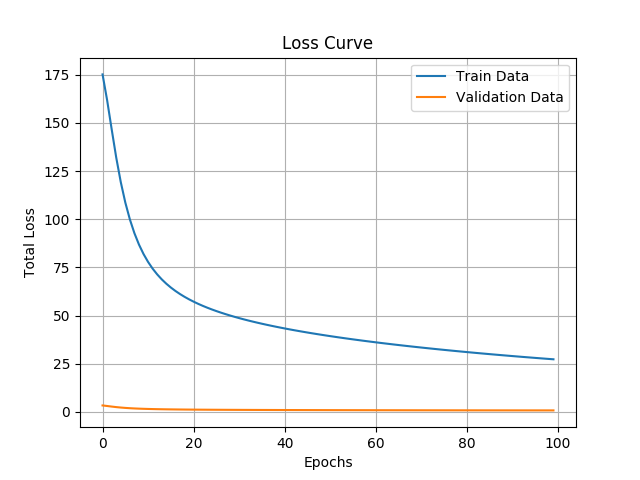
\includegraphics[width=0.5\textwidth]{Assignments/HW5/plots/q3_fcn_nist36_e3_loss.png}} &
{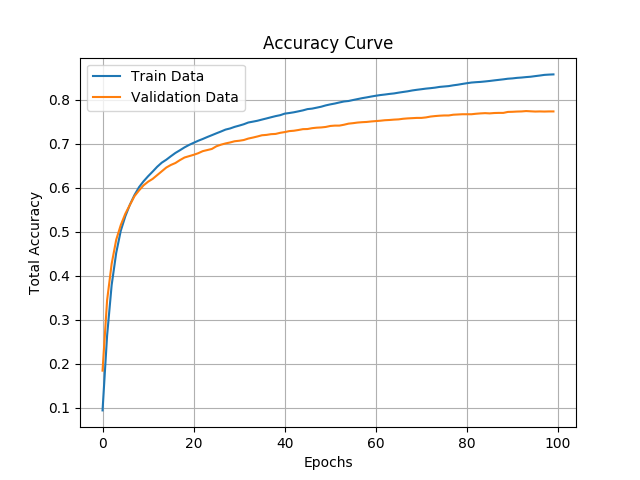
\includegraphics[width=0.5\textwidth]{Assignments/HW5/plots/q3_fcn_nist36_e3_accuracy.png}}
\end{tabular}
\caption{Loss and accuracy curves for learning rate = 1e-3}
\end{figure}

\begin{center}
\begin{BVerbatim}
Train Accuracy: 0.8575
Validation Accuracy: 0.7733
Test Accuracy: 0.7794
\end{BVerbatim}
\end{center}
\bigskip

\begin{figure}[!ht]
\centering
\begin{tabular}{cc}
{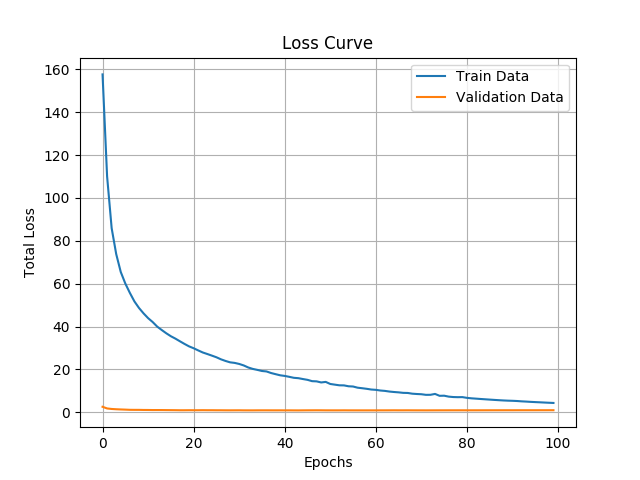
\includegraphics[width=0.5\textwidth]{Assignments/HW5/plots/q3_fcn_nist36_e2_loss.png}} &
{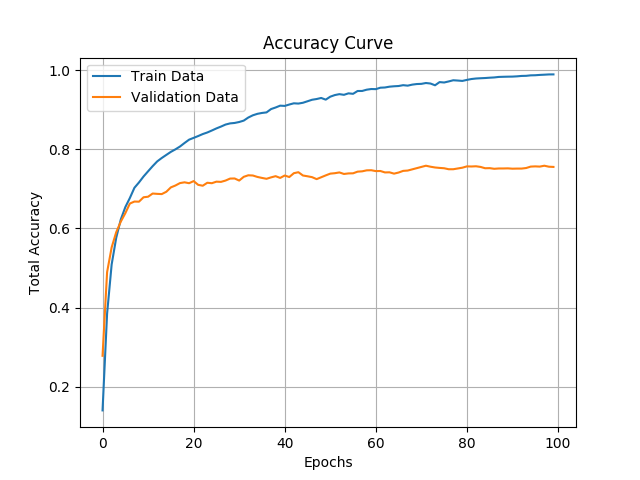
\includegraphics[width=0.5\textwidth]{Assignments/HW5/plots/q3_fcn_nist36_e2_accuracy.png}}
\end{tabular}
\caption{Loss and accuracy curves for learning rate = 1e-2}
\end{figure}

\begin{center}
\begin{BVerbatim}
Train Accuracy: 0.9893
Validation Accuracy: 0.7555
Test Accuracy: 0.7644
\end{BVerbatim}
\end{center}
\clearpage

\begin{figure}[!ht]
\centering
\begin{tabular}{cc}
{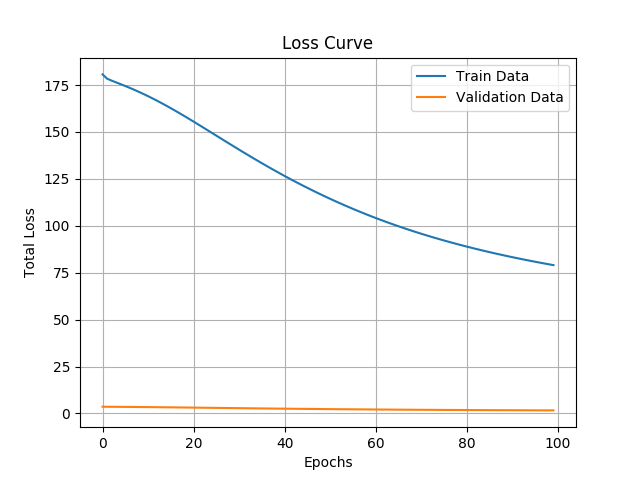
\includegraphics[width=0.5\textwidth]{Assignments/HW5/plots/q3_fcn_nist36_e4_loss.png}} &
{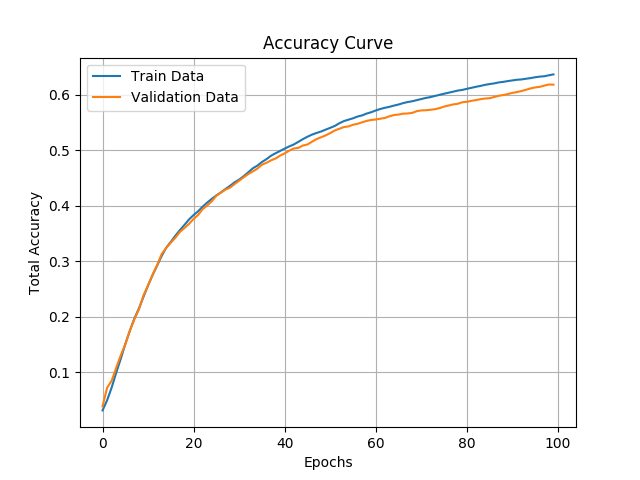
\includegraphics[width=0.5\textwidth]{Assignments/HW5/plots/q3_fcn_nist36_e4_accuracy.png}}
\end{tabular}
\caption{Loss and accuracy curves for learning rate = 1e-4}
\end{figure}

\begin{center}
\begin{BVerbatim}
Train Accuracy: 0.6371
Validation Accuracy: 0.6186
Test Accuracy: 0.6183
\end{BVerbatim}
\end{center}

\subsection{Weights Visualization}
Certain patterns can be observed in the weights after training. The corners and the regions near the edges seem to be low frequency or flat with less features learned and in the center region, we can see some visible strokes of the letters and numbers which look somewhat averaged over the dataset. The initial weights have no patterns in them as they are randomly initialized.\\
\begin{figure}[!ht]
\centering
\begin{tabular}{c}
{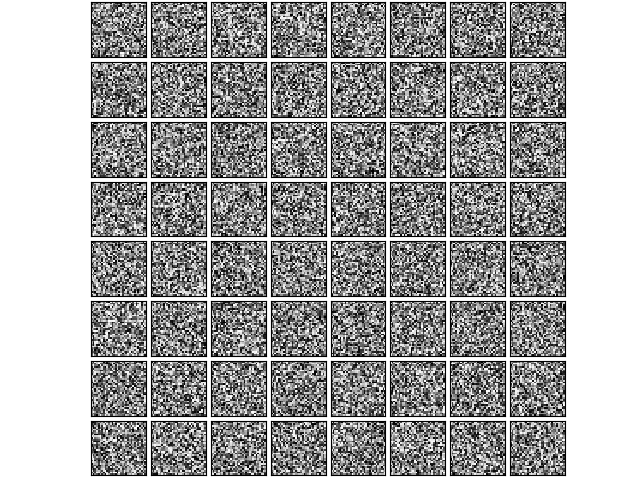
\includegraphics[width=0.8\textwidth]{Assignments/HW5/images/q3_initial.png}}
\end{tabular}
\caption{First layer weights immediately after initialization}
\end{figure}

\begin{figure}[!ht]
\centering
\begin{tabular}{c}
{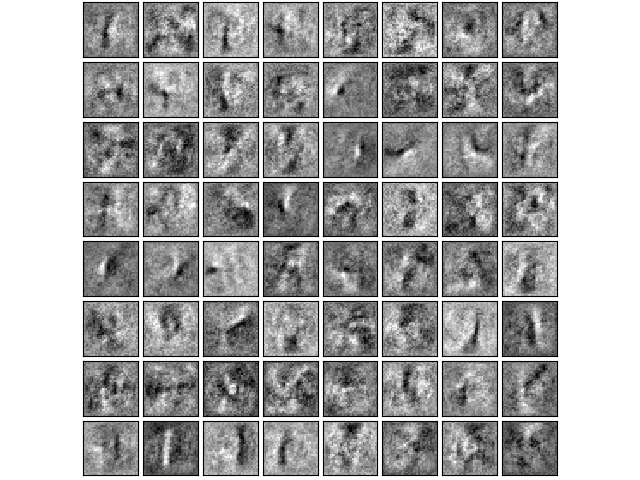
\includegraphics[width=0.8\textwidth]{Assignments/HW5/images/q3_final_e3.png}}
\end{tabular}
\caption{First layer weights after training for 100 epochs with learning rate 1e-3}
\end{figure}

\subsection{Confusion Matrix}
\begin{figure}[!ht]
\centering
\begin{tabular}{c}
{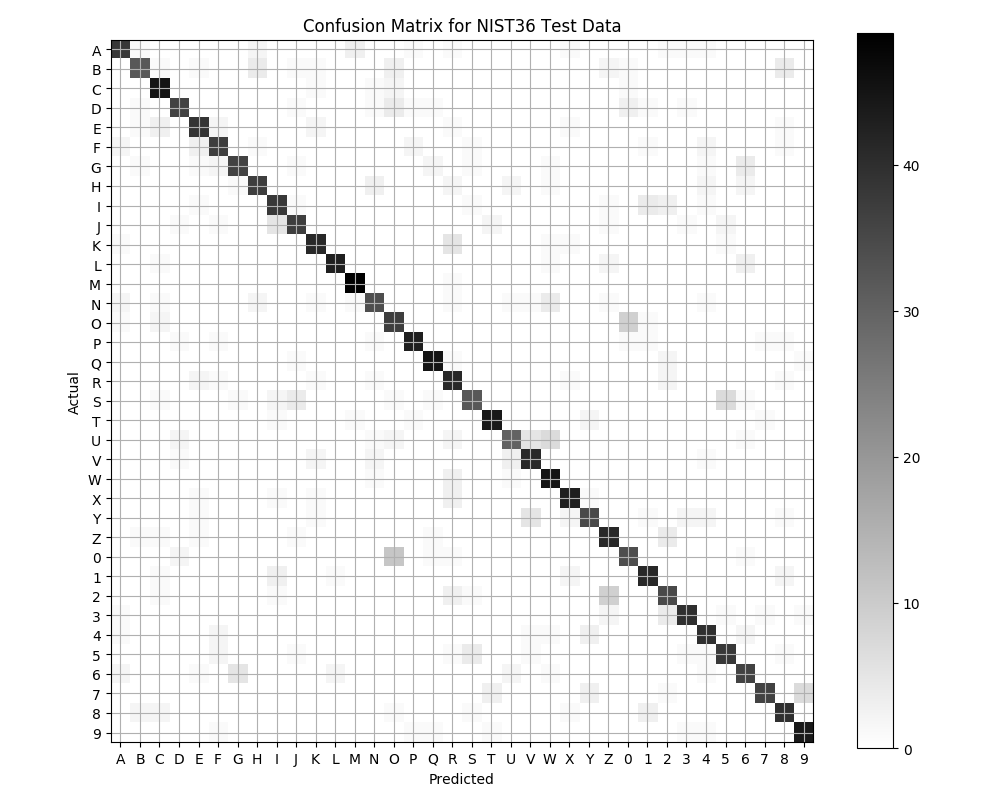
\includegraphics[width=0.74\textwidth]{Assignments/HW5/images/q3_conf_e3.png}}
\end{tabular}
\caption{Confusion matrix on the NIST36 test dataset after training 100 epochs with learning rate 1e-3. The top few pairs that are commonly confused are letter 'O' and number '0', '2' and 'Z', '5' and 'S', '6' and 'G', 'K' and 'R' which were expected.}
\end{figure}

\section{Extract Text from Images}
\subsection{Assumptions}
\begin{enumerate}
    \item Firstly, we assume that the characters extracted are very similar in structure to characters from the NIST36 dataset that we trained. This includes the stroke width, overall size and trivially, the style of writing. Another assumption is that the pixel values of the extracted characters are similar to the ones in the dataset, however the dataset does not have perfect binary black-and-white images upon inspection.
    \item The second assumption would be that, the text extraction or the cropped image is perfect without any noises or parts of neighbouring characters. This is true in most cases, except a few extractions.
\end{enumerate}

\begin{figure}[!ht]
\centering
\begin{tabular}{ccc}
{
\includegraphics[width=0.1\textwidth]{Assignments/HW5/images/01_list_31.png}} &
{
\includegraphics[width=0.1\textwidth]{Assignments/HW5/images/01_list_71.png}} &
{
\includegraphics[width=0.1\textwidth]{Assignments/HW5/images/02_letters_00.png}}
\end{tabular}
\caption{Example images where character detection might fail}
\end{figure}

In the first two images above, the characters look very ambiguous and in the first and last image, the stroke widths are slightly different than in the dataset and these images might fail to be detected correctly.

\subsection{Text Extraction}
Code implemented.

\subsection{Text Extraction Results}
\begin{figure}[!ht]
\centering
\begin{tabular}{ccc}
{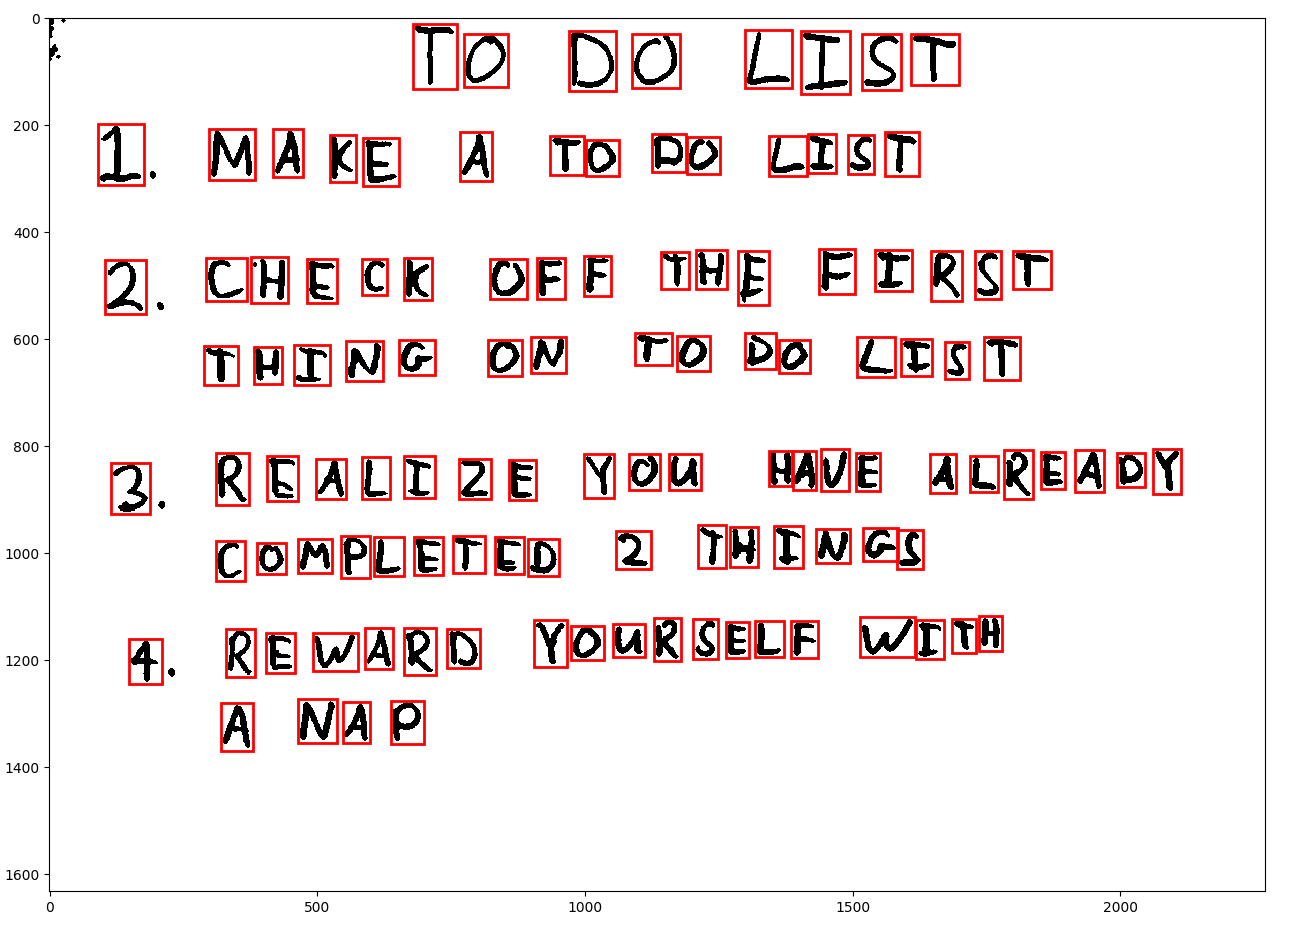
\includegraphics[width=0.82\textwidth]{Assignments/HW5/images/q4-box1.png}}
\end{tabular}
\caption{Text extraction results on 01\_list.jpg}
\end{figure}

\begin{figure}[!ht]
\centering
\begin{tabular}{ccc}
{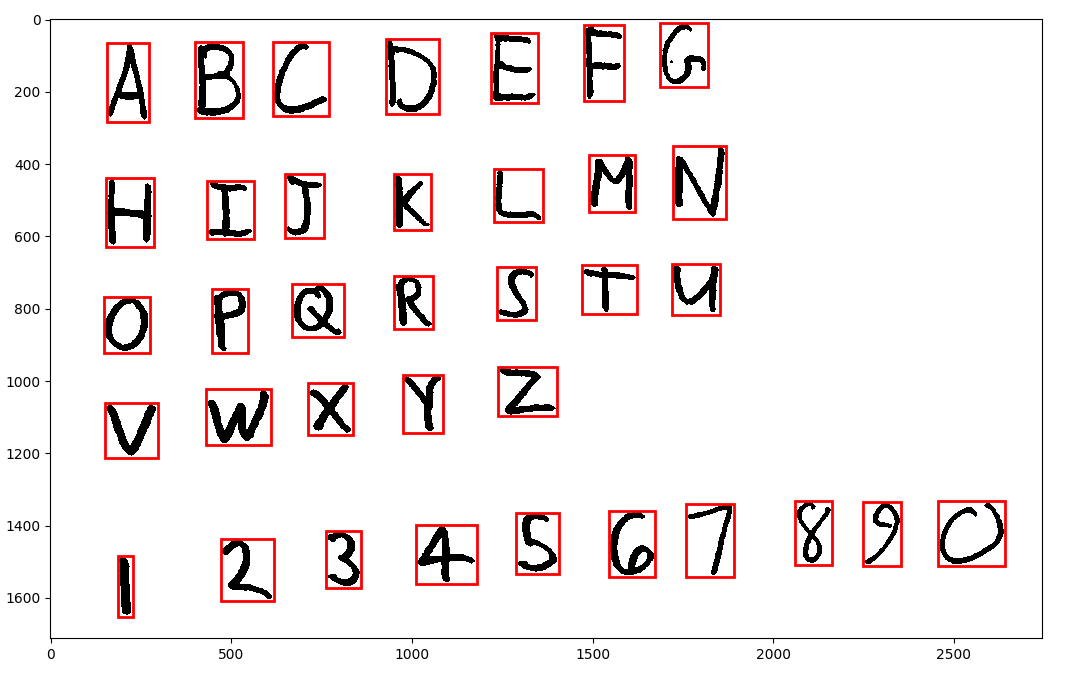
\includegraphics[width=0.75\textwidth]{Assignments/HW5/images/q4-box2.png}}
\end{tabular}
\caption{Text extraction results on 02\_letters.jpg}
\end{figure}

\begin{figure}[!ht]
\centering
\begin{tabular}{ccc}
{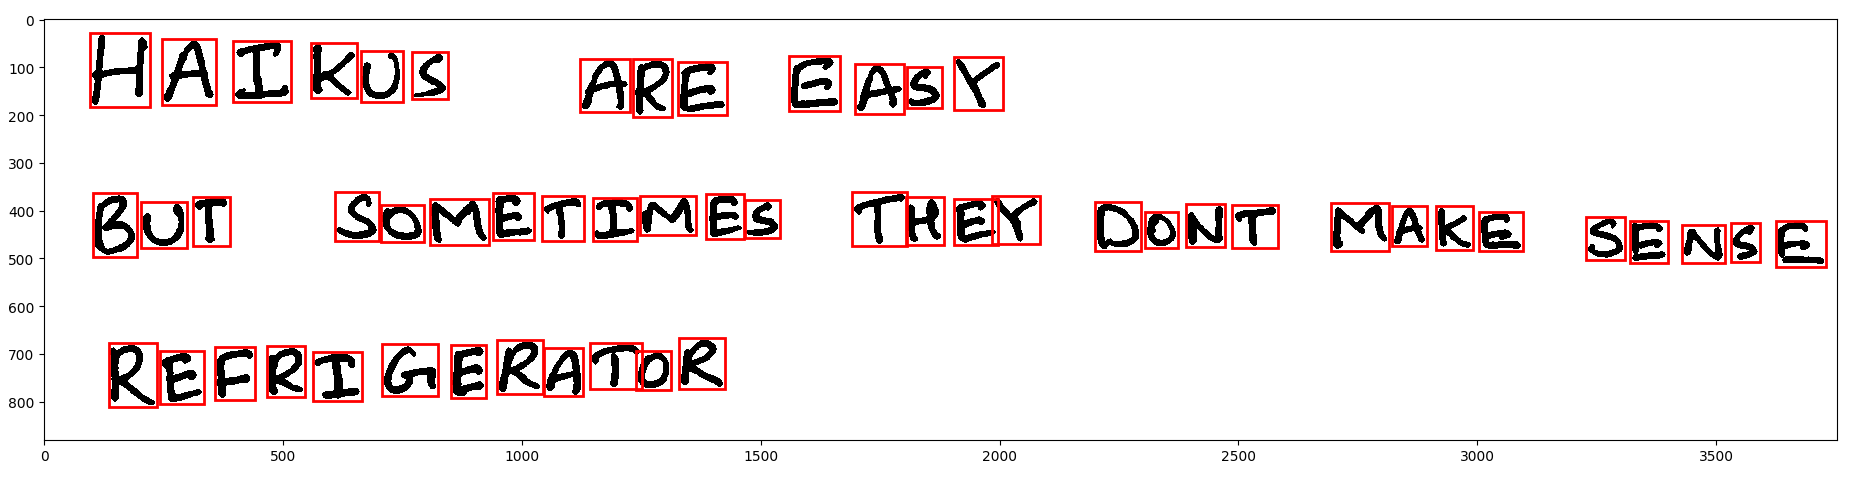
\includegraphics[width=0.82\textwidth]{Assignments/HW5/images/q4-box3.png}}
\end{tabular}
\caption{Text extraction results on 03\_haiku.jpg}
\end{figure}

\begin{figure}[!ht]
\centering
\begin{tabular}{ccc}
{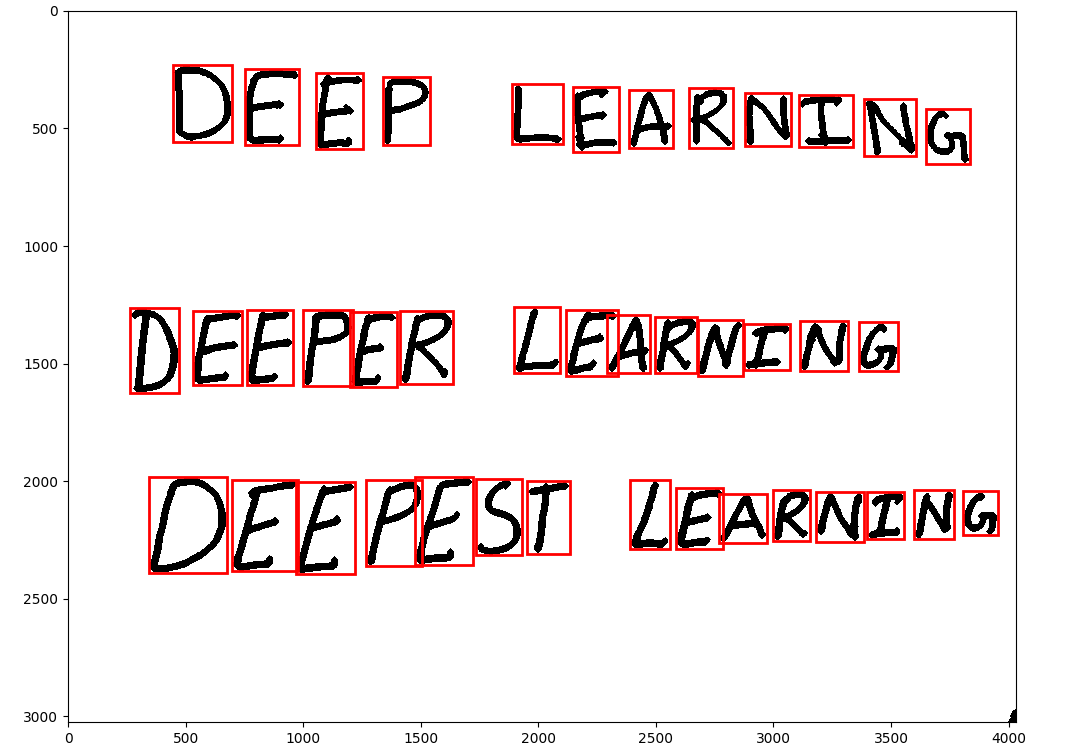
\includegraphics[width=0.75\textwidth]{Assignments/HW5/images/q4-box4.png}}
\end{tabular}
\caption{Text extraction results on 04\_deep.jpg}
\end{figure}

\begin{figure}[!ht]
\centering
\begin{tabular}{c}
{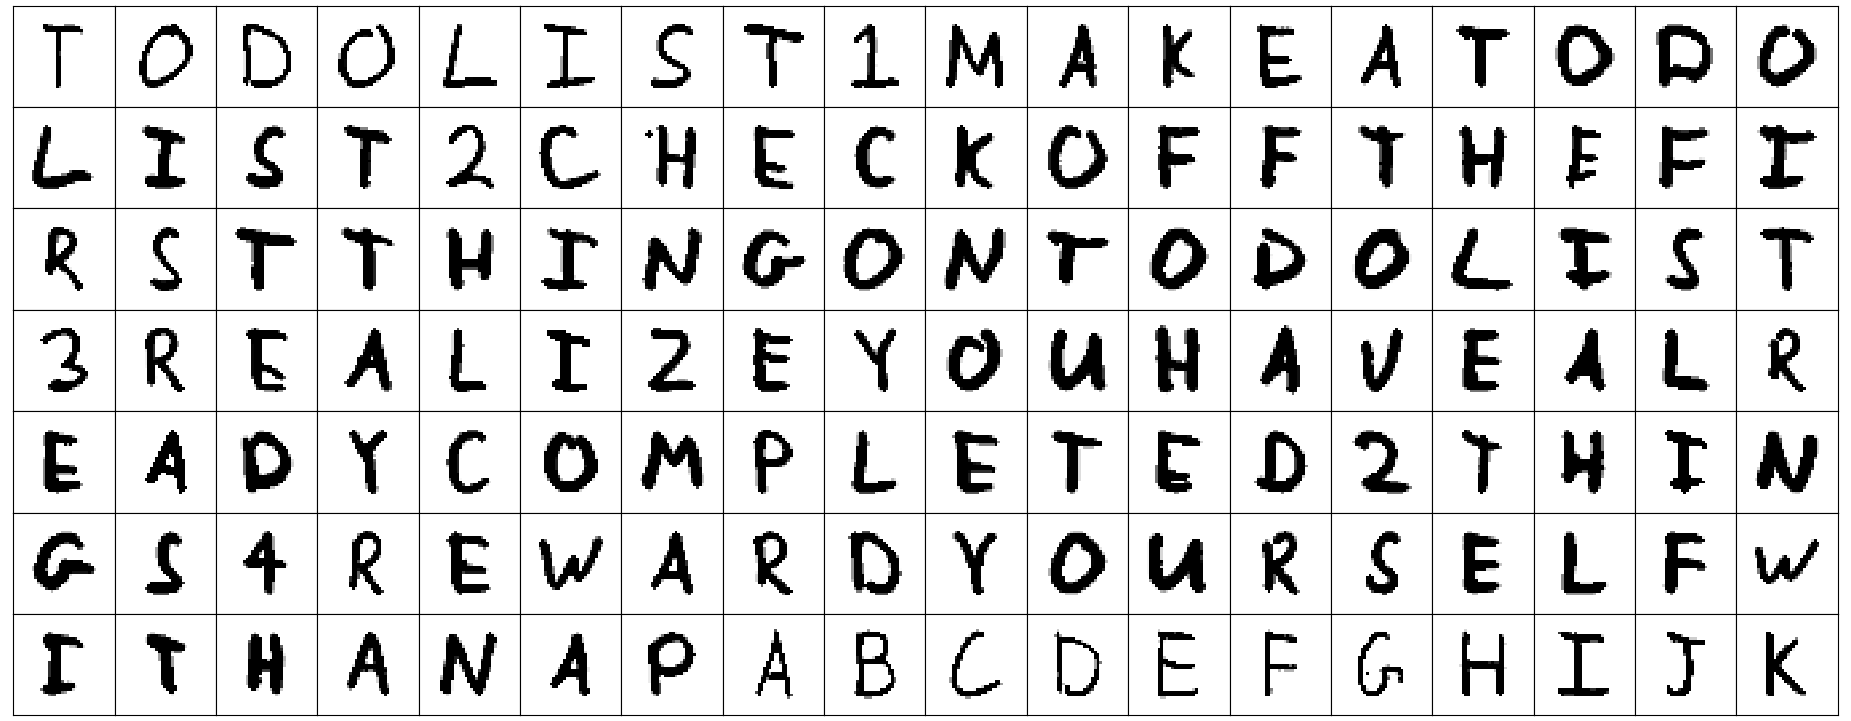
\includegraphics[width=0.8\textwidth]{Assignments/HW5/images/q4-text1.png}} \\
{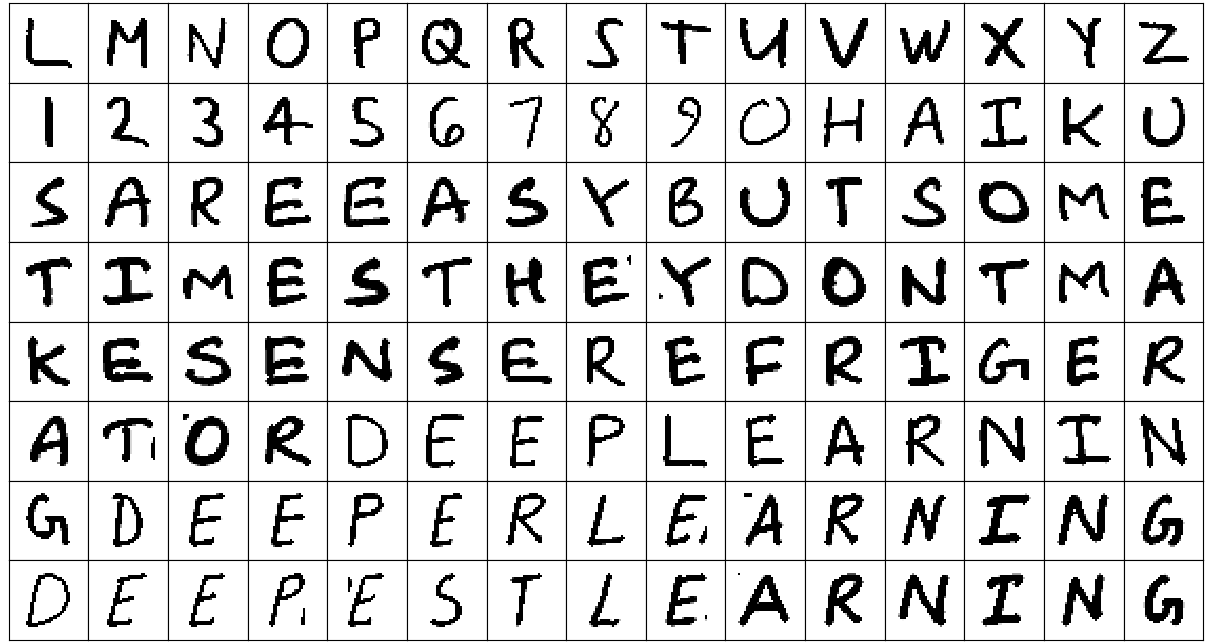
\includegraphics[width=0.8\textwidth]{Assignments/HW5/images/q4-test2.png}}
\end{tabular}
\caption{Text extraction results after cropping and padding}
\end{figure}

\subsection{Text Detection Results}
\begin{figure}[!ht]
\centering
\begin{BVerbatim}
T0 D0 LIST
I MAKE A TO 2O LIST
2 CHREK OFF THE FIRST
THING 0N T0 O0 LI5T
3 RFALIZE Y0U HAVE ALREADT
C0MPLETED 2 THINGS
4 REWARD X0URSELF WITH
A NAP

Accuracy: 85.22%
\end{BVerbatim}
\caption{Text detection results and accuracy for 01\_list.jpg}
\end{figure}

\begin{figure}[!ht]
\centering
\begin{BVerbatim}
2BCDEFG
HIJKLMN
0PQR5TW
VWXYZ
1Z3MS6789O

Accuracy: 77.78%
\end{BVerbatim}
\caption{Text detection results and accuracy for 02\_letters.jpg}
\end{figure}

\begin{figure}[!ht]
\centering
\begin{BVerbatim}
HAIKUS ARE EASY
BUT SQMETIMES TREX DONT MAKE SEMQE
REFRIGERAT0R

Accuracy: 88.89%
\end{BVerbatim}
\caption{Text detection results and accuracy for 03\_haiku.jpg}
\end{figure}

\begin{figure}[!ht]
\centering
\begin{BVerbatim}
DEEP LEARMING
DEEPER LEARKIM6
DEEREST LEARNIN6

Accuracy: 85.37%
\end{BVerbatim}
\caption{Text detection results and accuracy for 04\_deep.jpg}
\end{figure}

\section{Image Compression with Autoencoders}
\subsection{Building the Autoencoder}
Code implemented.

\subsection{Training the Autoencoder}
\begin{figure}[!ht]
\centering
\begin{tabular}{c}
{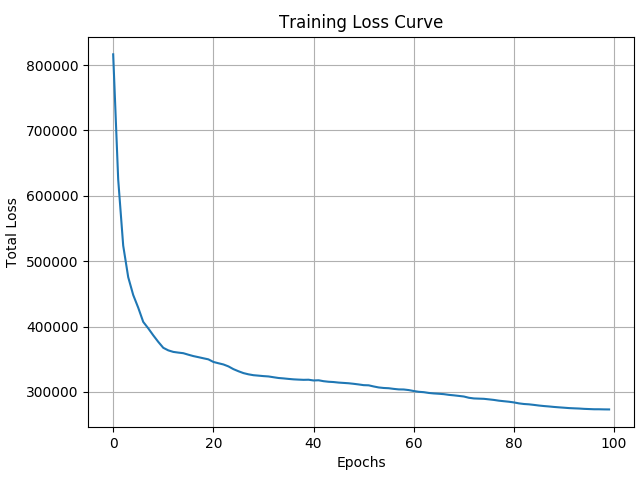
\includegraphics[width=0.8\textwidth]{Assignments/HW5/plots/q5_loss.png}}
\end{tabular}
\caption{Training loss curve for the Autoencoder}
\end{figure}

It can be seen that the training loss decreases as the training progresses with a initial steep drop and a very relaxed or flat drop in loss towards the end.

\subsection{Evaluating the Autoencoder}
\subsubsection{}
\begin{figure}[!ht]
\centering
\begin{tabular}{ccc}
{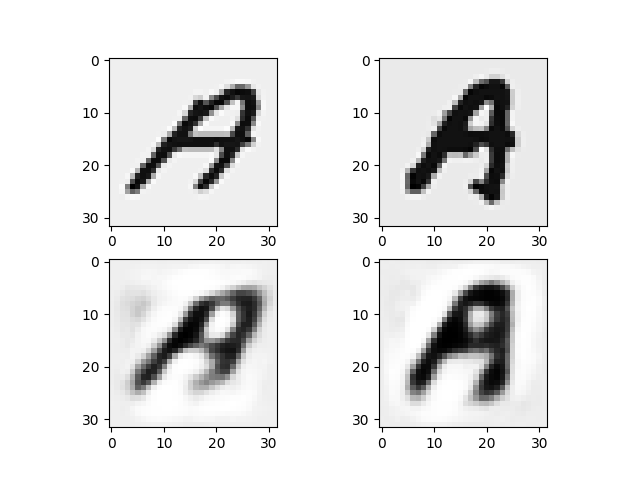
\includegraphics[width=0.3\textwidth]{Assignments/HW5/images/q5_1.png}} &
{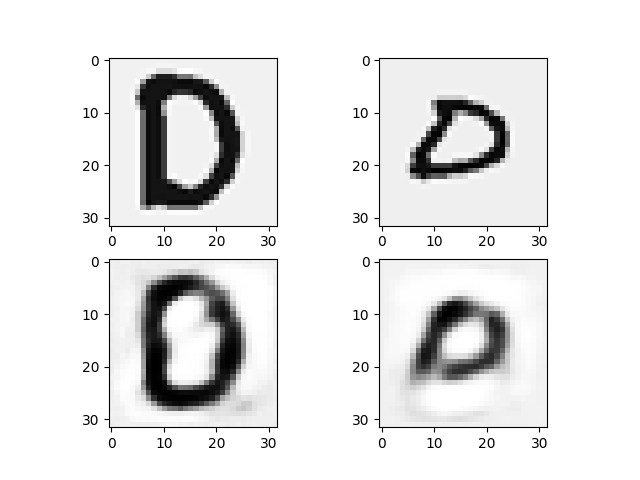
\includegraphics[width=0.3\textwidth]{Assignments/HW5/images/q5_2.png}} &
{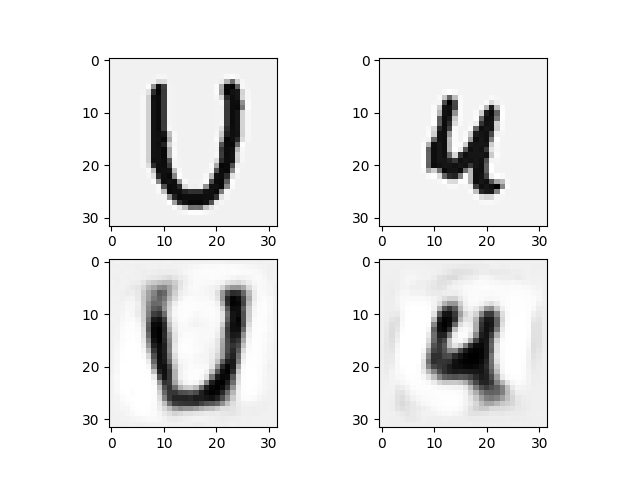
\includegraphics[width=0.3\textwidth]{Assignments/HW5/images/q5_3.png}}
\end{tabular}
\begin{tabular}{cc}
{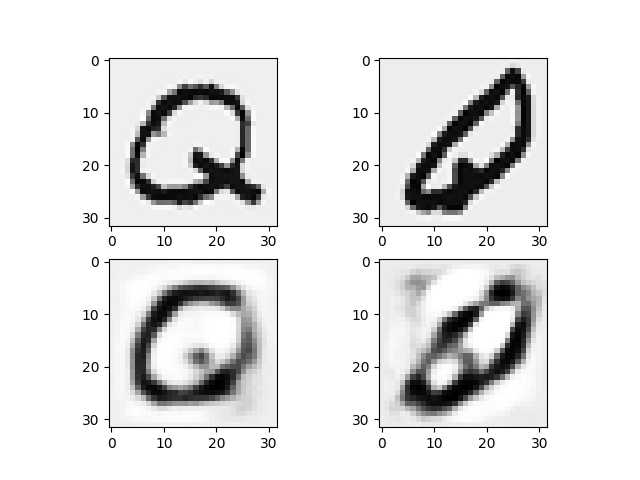
\includegraphics[width=0.3\textwidth]{Assignments/HW5/images/q5_4.png}} &
{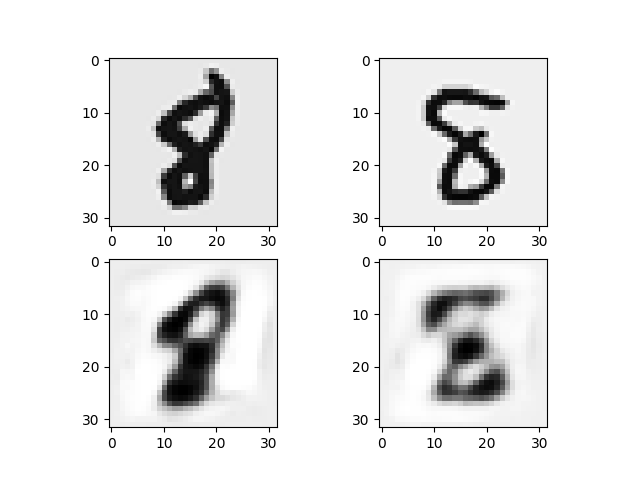
\includegraphics[width=0.3\textwidth]{Assignments/HW5/images/q5_5.png}}
\end{tabular}
\caption{Reconstruction results of the Autoencoder for five classes from the NIST36 test dataset}
\end{figure}

The reconstruction results look blurry and the loss in high frequency components and features is clearly visible. This is because we are reducing the dimensionality at the bottleneck of the Autoencoder.

\subsubsection{}
The average Peak Signal-Noise Ratio (PSNR) across all the validation images was \textbf{15.9145}.

\section{Comparing against PCA}
\subsection{Projection Matrix}
The size of the projection matrix is $\mathbf{32 \times 1024}$ and its rank is $\mathbf{32}$. The reconstruction on test images is shown in \textit{Figure 19}.

\subsection{PCA Reconstruction Results}
The reconstruction results look blurry and the loss in high frequency components and features is clearly visible. This is because we are reducing the dimensionality and taking only 32 principal components. Compared to Autoencoder, the text reconstruction is more blurry and the background reconstruction is not as good as Autoencoder.

\begin{figure}[!ht]
\centering
\begin{tabular}{ccc}
{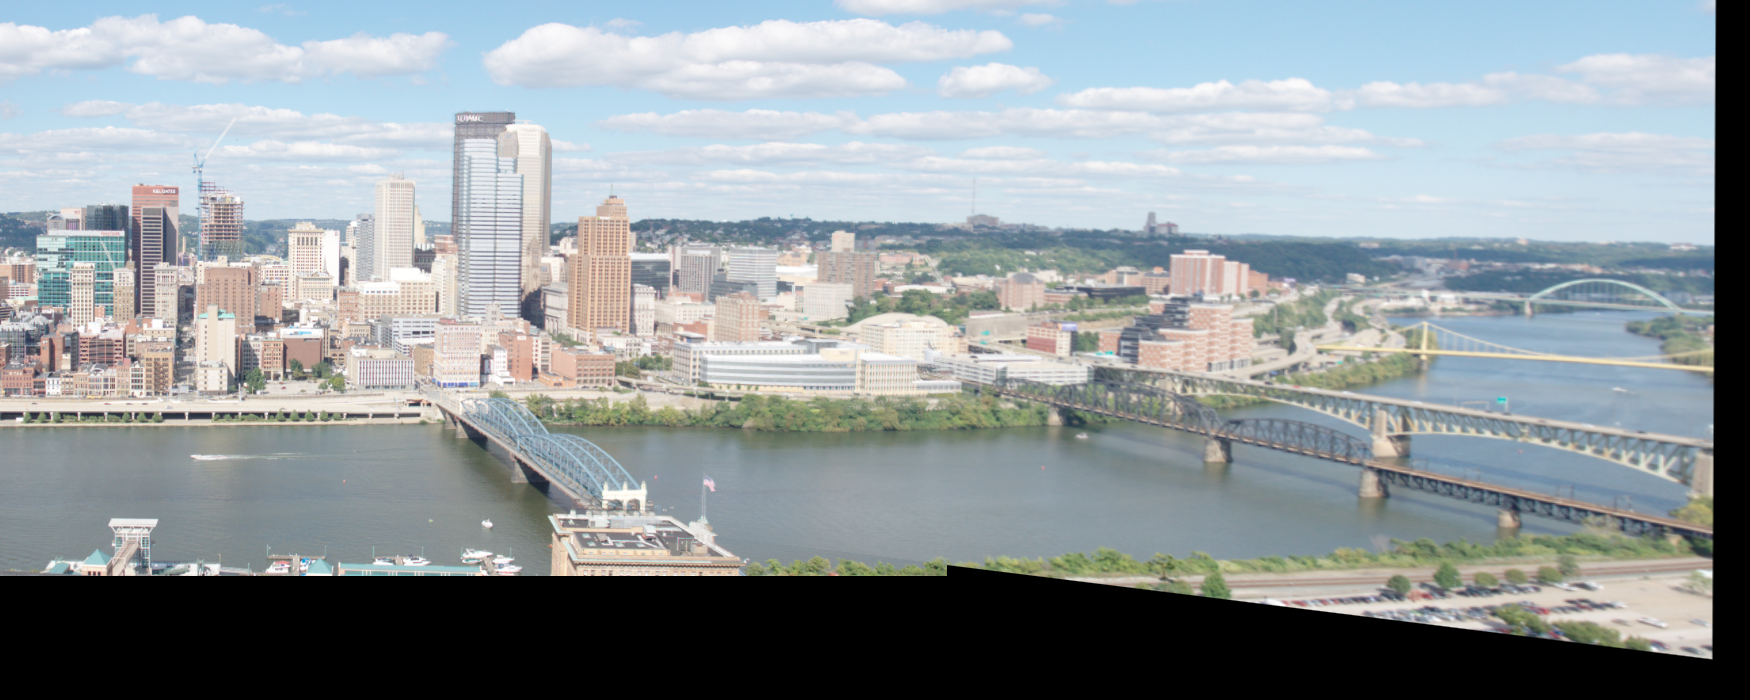
\includegraphics[width=0.3\textwidth]{Assignments/HW5/images/q6_1.png}} &
{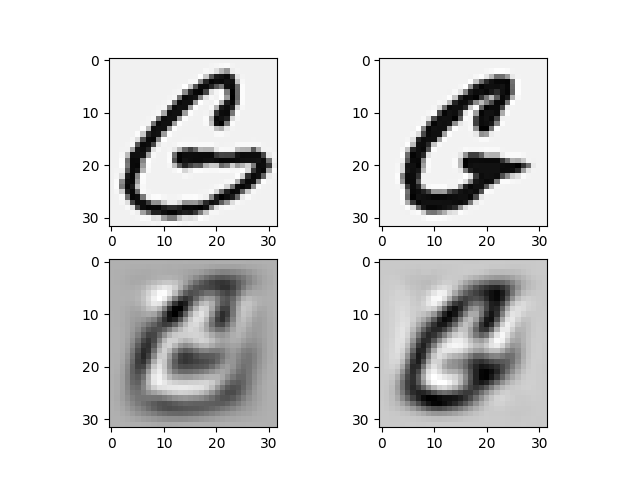
\includegraphics[width=0.3\textwidth]{Assignments/HW5/images/q6_2.png}} &
{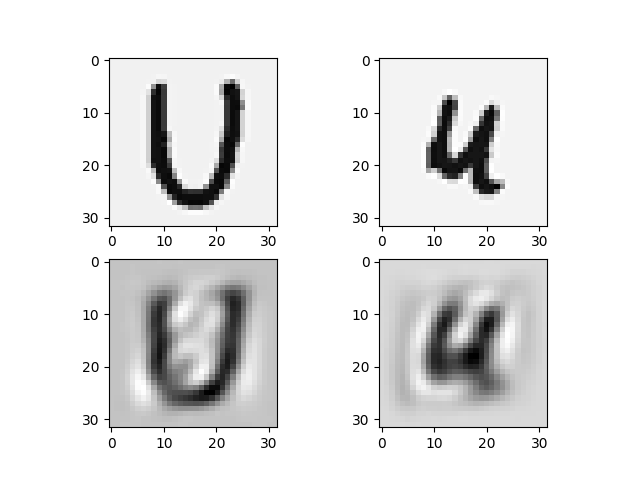
\includegraphics[width=0.3\textwidth]{Assignments/HW5/images/q6_3.png}}
\end{tabular}
\begin{tabular}{cc}
{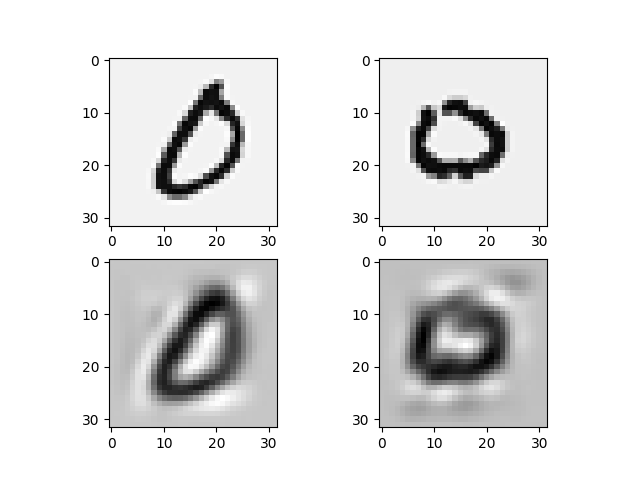
\includegraphics[width=0.3\textwidth]{Assignments/HW5/images/q6_4.png}} &
{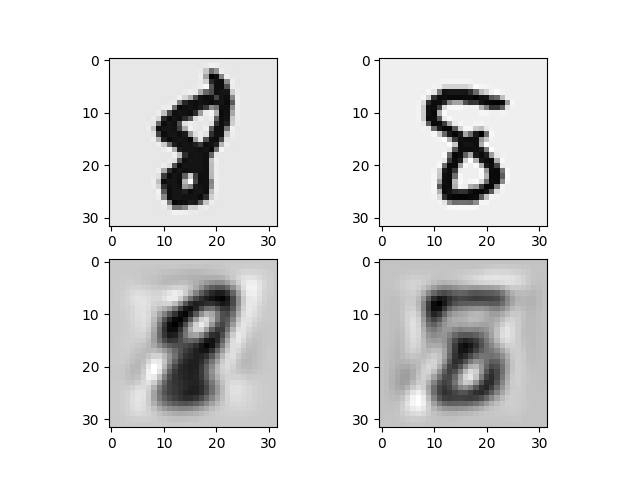
\includegraphics[width=0.3\textwidth]{Assignments/HW5/images/q6_5.png}}
\end{tabular}
\caption{Reconstruction results of PCA for the same five classes from the NIST36 test dataset}
\end{figure}

\subsection{Evaluating PCA}
The average Peak Signal-Noise Ratio (PSNR) across all the validation images was \textbf{16.2839}. The PCA PSNR was slightly better than the Autoencoder's PSNR. However, on visualization of the reconstructed images, Autoencoder seems to perform better. This is also true because the Autoencoder has non-linearities introduced by the ReLU activation function, which helps to learn the classification function better, compared to dealing with just linear operations using SVD in PCA. Furthermore, the number of learned parameters in Autoencoder is almost double that of PCA. 

But as per the PSNR, PCA is better and the reason for this could be that in Autoencoder, the high frequency component reconstruction is more visible compared to PCA, although not prefect. These imperfect higher frequency components may contribute to more noise and thus the PSNR of PCA could be better than the PSNR of Autoencoder.

\subsection{Number of Learned Parameters}
The number of learned parameters for Autoencoder including the weights and biases is \textbf{68,704}.\\
The number of learned parameters for PCA is \textbf{32,768}. \\
The reasons for better performance are already discussed above in \textit{6.3}.

\clearpage
\section{PyTorch}
\subsection{Train a Neural Network in PyTorch
}
\subsubsection{Fully Connected Network with NIST36 Dataset}
\begin{figure}[!ht]
\centering
\begin{tabular}{cc}
{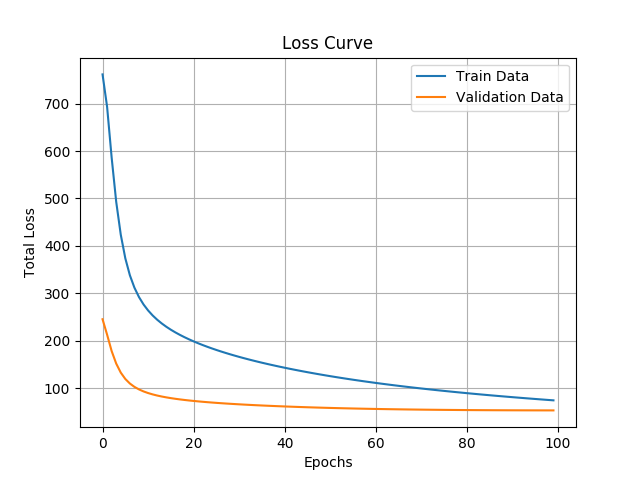
\includegraphics[width=0.5\textwidth]{Assignments/HW5/plots/fcn_nist36_loss.png}} &
{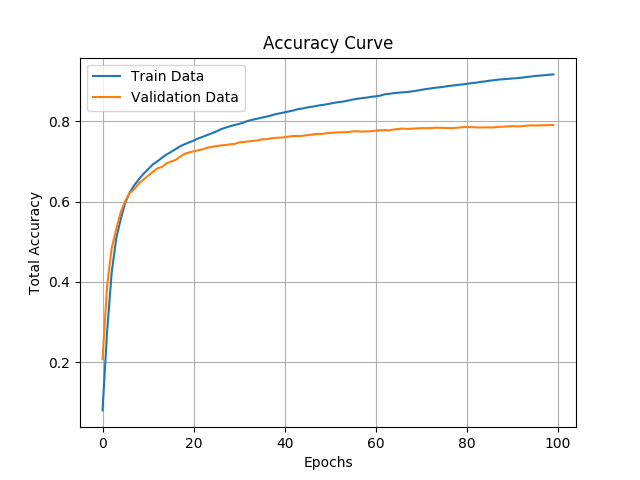
\includegraphics[width=0.5\textwidth]{Assignments/HW5/plots/fcn_nist36_accuracy.png}}
\end{tabular}
\caption{Loss and accuracy curves for Fully Connected Network with NIST36 Dataset}
\end{figure}

\subsubsection{Convolution Neural Network (LeNet-5) with MNIST Dataset}
\begin{figure}[!ht]
\centering
\begin{tabular}{cc}
{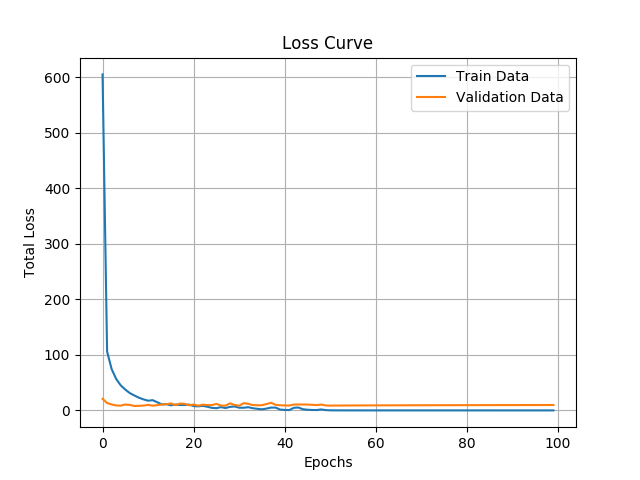
\includegraphics[width=0.5\textwidth]{Assignments/HW5/plots/cnn_mnist_loss.png}} &
{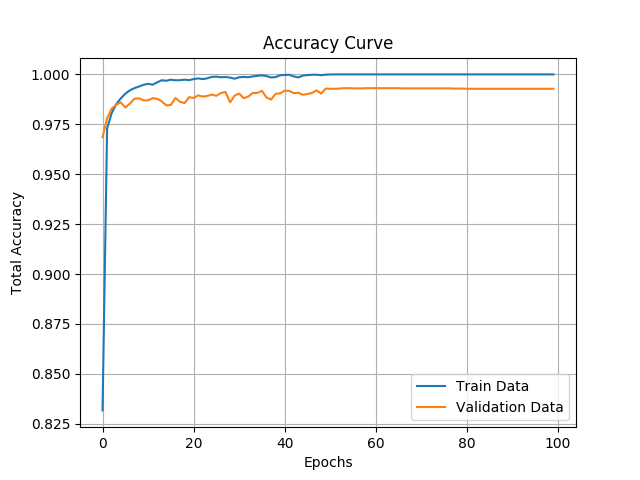
\includegraphics[width=0.5\textwidth]{Assignments/HW5/plots/cnn_mnist_accuracy.png}}
\end{tabular}
\caption{Loss and accuracy curves for Convolution Neural Network (LeNet-5) with MNIST Dataset}
\end{figure}

\clearpage
\subsubsection{Convolution Neural Network (LeNet-5) with NIST36 Dataset}
\begin{figure}[!ht]
\centering
\begin{tabular}{cc}
{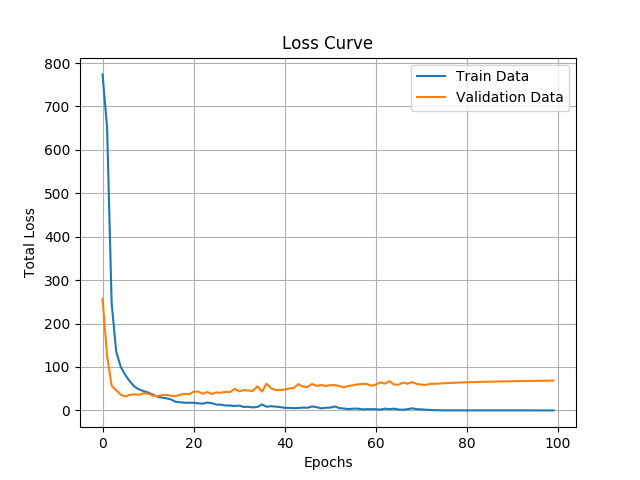
\includegraphics[width=0.5\textwidth]{Assignments/HW5/plots/cnn_nist36_loss.png}} &
{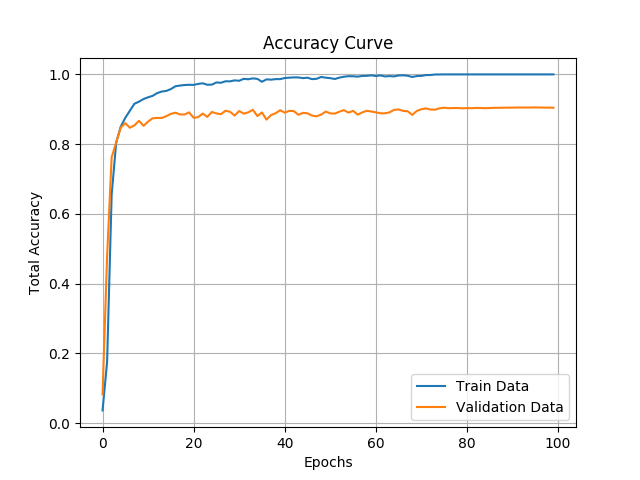
\includegraphics[width=0.5\textwidth]{Assignments/HW5/plots/cnn_nist36_accuracy.png}}
\end{tabular}
\caption{Loss and accuracy curves for Convolution Neural Network (LeNet-5) with NIST36 Dataset}
\end{figure}

\subsubsection{Convolution Neural Network (LeNet-5) with EMNIST Dataset}
\begin{figure}[!ht]
\centering
\begin{tabular}{cc}
{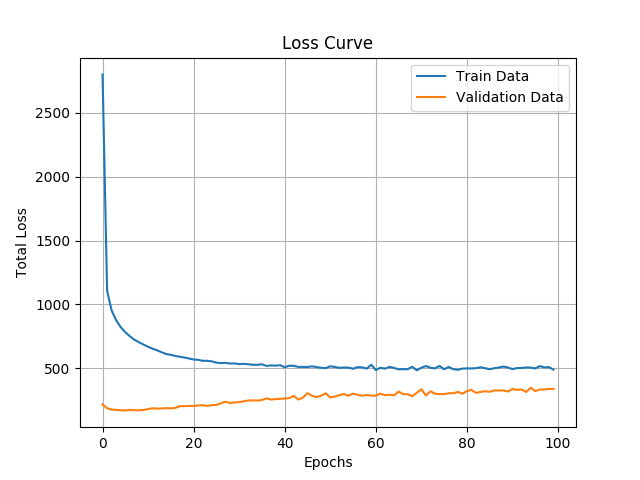
\includegraphics[width=0.5\textwidth]{Assignments/HW5/plots/cnn_emnist_loss.png}} &
{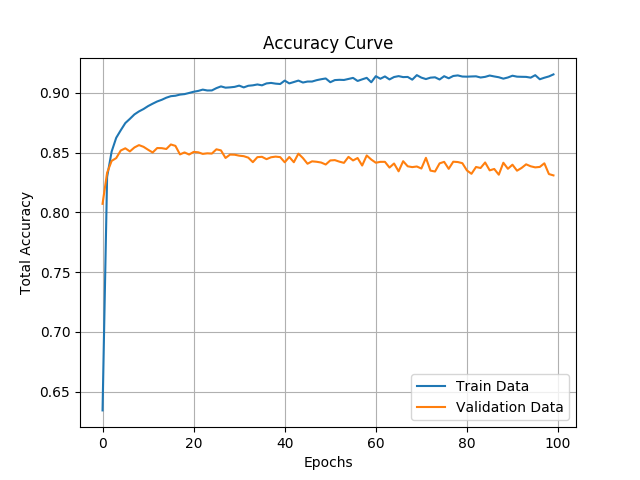
\includegraphics[width=0.5\textwidth]{Assignments/HW5/plots/cnn_emnist_accuracy.png}}
\end{tabular}
\caption{Loss and accuracy curves for Convolution Neural Network (LeNet-5) with EMNIST Dataset}
\end{figure}

\begin{figure}[!ht]
\centering
\begin{BVerbatim}
JD DO LI5T
I MARE A TO DO LIST
2 CHECK OFF THE FIfST
THINQ ON TO DO LZST
3 REAEE2E YOU HAVE AfREADY
COMPLErED 2 THINGS
4 REWARD YOURSELF WITH
R NAP

Actual Accuracy: 87.83%
Absolute Accuracy: 87.83%
\end{BVerbatim}
\caption{Text detection results and accuracy with LeNet-5 for 01\_list.jpg}
\end{figure}

Two accuracies are reported here. The actual accuracy is case sensitive and the absolute accuracy is reported after converting all labels and predictions to upper-case.

\begin{figure}[!ht]
\centering
\begin{BVerbatim}
ABCDEfG
HIJKLMN
OPQRStY
VWXYZ
12345G78gD

Actual Accuracy: 83.33%
Absolute Accuracy: 88.89%
\end{BVerbatim}
\caption{Text detection results and accuracy with LeNet-5 for 02\_letters.jpg}
\end{figure}

\begin{figure}[!ht]
\centering
\begin{BVerbatim}
HAIKUS ARE EASY
BUT SOMETIMES THEY DONt MAKE SEnGE
REfRI6ERAtOR

Actual Accuracy: 88.89%
Absolute Accuracy: 96.30%
\end{BVerbatim}
\caption{Text detection results and accuracy with LeNet-5 for 03\_haiku.jpg}
\end{figure}

\begin{figure}[!ht]
\centering
\begin{BVerbatim}
DEEP LEARNING
dEEPER LEARNIN6
DEERE5J LEARNZNG

Actual Accuracy: 85.37%
Absolute Accuracy: 87.80%
\end{BVerbatim}
\caption{Text detection results and accuracy with LeNet-5 for 04\_deep.jpg}
\end{figure}

\subsection{Fine Tuning}
\subsubsection{Fine Tuning Flowers-17 Dataset on SqueezeNet 1.1 vs Training LeNet-5 from Scratch}

The results of fine-tuning SqueezeNet 1.1 classifier (validation accuracy of 0.86) was much better than training LeNet-5 (validation accuracy of 0.49) from scratch. This was expected because SqueezeNet has a much deeper architecture and learns more features. Furthermore, SqueezeNet was trained on a much larger dataset, ImageNet compared to Oxford Flowers-17.

\begin{figure}[!ht]
\centering
\begin{tabular}{cc}
{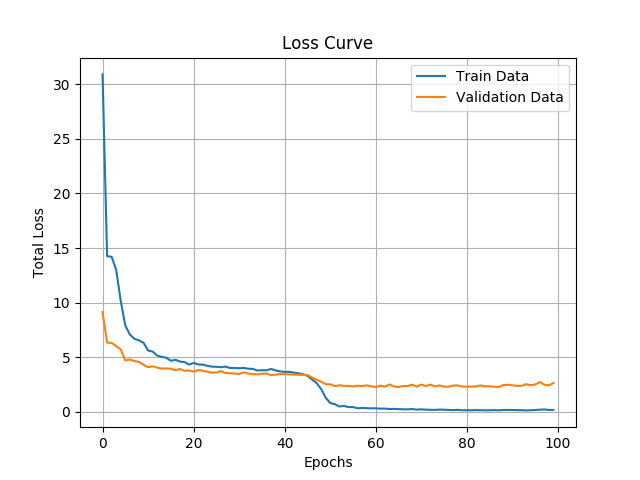
\includegraphics[width=0.5\textwidth]{Assignments/HW5/plots/squeezenet_loss.png}} &
{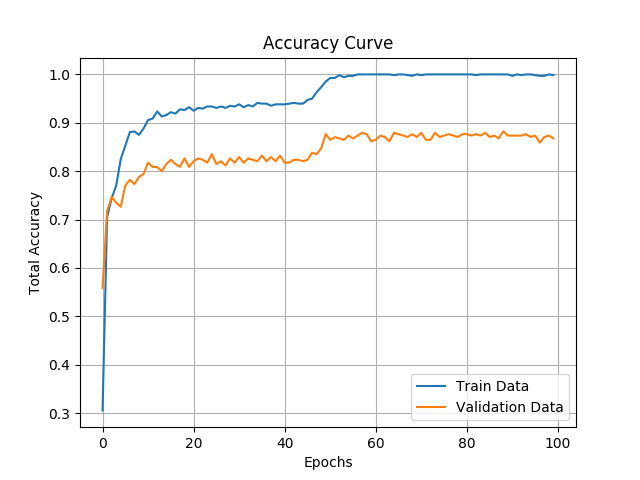
\includegraphics[width=0.5\textwidth]{Assignments/HW5/plots/squeezenet_accuracy.png}}
\end{tabular}
\caption{Loss and accuracy curves for fine-tuning SqueezeNet 1.1 with Flowers-17 Dataset}
\end{figure}

\begin{figure}[!ht]
\centering
\begin{tabular}{cc}
{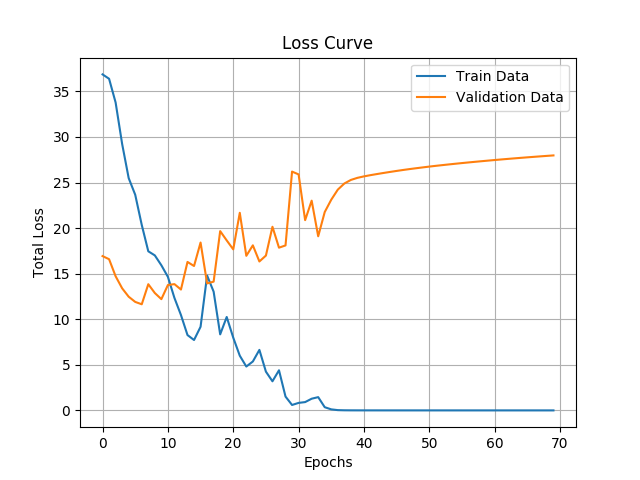
\includegraphics[width=0.5\textwidth]{Assignments/HW5/plots/lenet5_flowers_loss.png}} &
{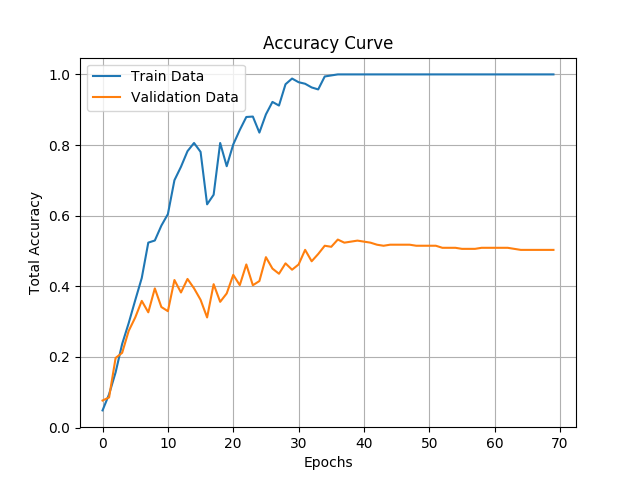
\includegraphics[width=0.5\textwidth]{Assignments/HW5/plots/lenet5_flowers_accuracy.png}}
\end{tabular}
\caption{Loss and accuracy curves for training LeNet-5 with Flowers-17 Dataset from scratch}
\end{figure}

\end{document} 